% !TEX encoding = UTF-8 Unicode

% Compilation using 'acmsmall.cls' - version 1.3 (March 2012), Aptara Inc.
% (c) 2010 Association for Computing Machinery (ACM)
%
% Questions/Suggestions/Feedback should be addressed to => "acmtexsupport@aptaracorp.com".
% Users can also go through the FAQs available on the journal's submission webpage.
%
% Steps to compile: latex, bibtex, latex, latex


\documentclass[prodmode,acmtochi]{acmsmall} % Aptara syntax

% Package to generate and customize Algorithm as per ACM style
\usepackage[ruled]{algorithm2e}
\renewcommand{\algorithmcfname}{ALGORITHM}
\SetAlFnt{\small}
\SetAlCapFnt{\small}
\SetAlCapNameFnt{\small}
\SetAlCapHSkip{0pt}
\IncMargin{-\parindent}

% Metadata Information
\acmVolume{9}
\acmNumber{4}
\acmArticle{39}
\acmYear{2010}
\acmMonth{3}

% Copyright
%\setcopyright{acmcopyright}
%\setcopyright{acmlicensed}
%\setcopyright{rightsretained}
%\setcopyright{usgov}
%\setcopyright{usgovmixed}
%\setcopyright{cagov}
%\setcopyright{cagovmixed}

% DOI
\doi{0000001.0000001}

%ISSN
\issn{1234-56789}

% Document starts
\begin{document}

% Page heads
\markboth{B. Harmon et al.}{Embodied Spatial Cognition in Tangible Computing}

% Title portion
\title{Embodied Spatial Cognition in Tangible Computing} % Spatial Performance in Tangible Computing 
\author{BRENDAN ALEXANDER HARMON
\affil{North Carolina State University}
ANNA PETRASOVA
\affil{North Carolina State University}
VACLAV PETRAS
\affil{North Carolina State University}
HELENA MITASOVA
\affil{North Carolina State University}
ROSS ​KENDALL MEENTEMEYER
\affil{North Carolina State University}}

\begin{abstract}
\ldots


% embodied cognition
% tangible interaction
% improve spatial performance
% design of tangible landscape
% experiments to test spatial performance

\end{abstract}

%
% The code below should be generated by the tool at
% http://dl.acm.org/ccs.cfm
% Please copy and paste the code instead of the example below. 
%
\begin{CCSXML}
<ccs2012>
<concept>
<concept_id>10003120.10003121</concept_id>
<concept_desc>Human-centered computing~Human computer interaction (HCI)</concept_desc>
<concept_significance>500</concept_significance>
</concept>
<concept>
<concept_id>10003120.10003121.10003122.10011749</concept_id>
<concept_desc>Human-centered computing~Laboratory experiments</concept_desc>
<concept_significance>500</concept_significance>
</concept>
</ccs2012>
\end{CCSXML}

\ccsdesc[500]{Human-centered computing~Human computer interaction (HCI)}
\ccsdesc[500]{Human-centered computing~Laboratory experiments}
%
% End generated code
%

\keywords{Human-computer interaction, tangible interfaces, interaction design, physical computation, embodied cognition, spatial thinking, geospatial modeling}

\acmformat{Brendan A. Harmon, Anna Petrasova, Vaclav Petras, Helena Mitasova, and Ross K. Meentemeyer, 2016. Embodied Spatial Cognition in Tangible Computing.}
% At a minimum you need to supply the author names, year and a title.
% IMPORTANT:
% Full first names whenever they are known, surname last, followed by a period.
% In the case of two authors, 'and' is placed between them.
% In the case of three or more authors, the serial comma is used, that is, all author names
% except the last one but including the penultimate author's name are followed by a comma,
% and then 'and' is placed before the final author's name.
% If only first and middle initials are known, then each initial
% is followed by a period and they are separated by a space.
% The remaining information (journal title, volume, article number, date, etc.) is 'auto-generated'.

\begin{bottomstuff}
Author's addresses: B. A. Harmon {and} A. Petrasova {and} V. Petras {and} H. Mitasova {and} R. K. Meentemeyer, Center for Geospatial Analytics, North Carolina State University.
% ; G. H. Bressler, Department of Landscape Architecture, North Carolina State University.
\end{bottomstuff}

\maketitle


\section{Introduction}

We have designed Tangible Landscape -- a tangible interface powered by a geographic information system (GIS) -- 
that gives spatial data an interactive, physical form so that users can naturally feel it, see it, and shape it.
%
Our aim was to iteratively design and empirically test a tangible interface that augments spatial thinking and improves spatial performance. 
%
Spatial thinking can be embodied -- people can functionally think about space with their bodies by cognitively grasping objects and physically simulating it \cite{Kirsh2013}.
%
Theoretically tangible interfaces should improve spatial performance through embodied cognition by enabling natural modes of interaction \cite{Dourish2001}, offloading cognitive processes onto the body \cite{Kirsh2013}, and computationally augmenting spatial thinking \cite{Dror2008}. 
%
We designed Tangible Landscape to physically manifest digital data so that users can cognitively grasp the data as an extension of their bodies and automatically, immediately, and subconsciously interact with it. 
%
We conducted a series of experiments using quantitative methods including geospatial modeling, analysis, simulation, and statistics and qualitative methods including semi-structured interviews and direct observation
to test whether tangible interfaces can improve spatial performance. 
%
We also explored how users approached spatial problem solving using Tangible Landscape in a serious gaming event.

% Concept diagram / illustration

\pagebreak

\subsection{Spatial thinking}

Spatial thinking -- `the mental processes of representing, analyzing, and drawing inferences from spatial relations' \cite{Uttal2013} -- is used pervasively in everyday life % at a personal scale 
for tasks like recognizing things, manipulating things, interacting with others, and way-finding. 
%
Spatial thinking is also used extensively in science, technology, engineering, the arts, and math 
for tasks like 
simulating physical processes,
mapping and manipulating molecules,
designing circuits, 
designing buildings, 
shaping sculpture,
and studying topology. 
%
Given the importance of spatial thinking -- personally, academically, and professionally -- %how can we improve it? 
how can we effectively improve our spatial performance, our ability to perform tasks that require spatial thinking? 
% how can spatial performance, our ability to perform tasks that require spatial thinking, effectively be improved?

Many spatial tasks can be performed computationally 
enabling us to efficiently store, model, and analyze large sets of spatial data 
and solve complex spatiotemporal problems.
%
In engineering, design, and the arts 
computer-aided design (CAD) and 3D modeling software are used to interactively, computationally model, analyze, and animate complex spatial forms. 
%
In scientific computing spatial patterns and processes can be mathematically modeled, simulated, and optimized. 
%
Geographic information systems, for example, can be used to computationally store, model, analyze, simulate, and represent geospatial patterns and processes. 
%
The open source project GRASS GIS for example supports 
`geospatial data management and analysis, image processing, graphics and maps production, spatial modeling, and visualization' \cite{GRASS}. 
%\footnote{\url{https://grass.osgeo.org/}} 
%
% add more citations

Computing mediates and transforms spatial thinking, expanding, but also constraining what is possible.
%
While spatial computing can augment spatial thinking 
-- distributing or offloading cognitive processes through digital computation -- 
the logic of implementation,
the limits of what is computationally possible, 
and the modes of input and output
constrain how we reason. % citations
%
Furthermore, 
when it is difficult to interact with a computer, 
to input commands and parse the resulting output, 
one has to think harder and risks frustration and demotivation. % citations
% these cognitive costs and risks...
%
%Furthermore, 
%difficulty in interacting with a computer
%-- in inputing commands and parsing the resulting output --
%can add cognitive costs, generate frustration, and sap motivation. 

Unintuitive modes of human-computer interaction constrain how we think and add cognitive and emotional costs. 
%
The paradigmatic modes for interacting with computers today 
-- command line interfaces (CLI) and
graphical user interfaces (GUI)
%including touch interfaces
 -- 
require physical input from devices like mice, keyboards, digitizing pens, and touch screens, but
output %present %render
data visually as text or graphics. 



% disconnect between intention, action, and feedback

...\\

Imagine sculpting a volume in a 3D modeling program.

When sculpting a volume

There is a disconnect between intention, action, and feedback when one imagines a change, clicks with a mouse, and then sees the change on a display. 

% LIMITED TO VISUAL FEEDBACK

% CHALLENGES IN VISUALIZING COMPLEX FORMS/PATTERNS

% the disconnect between intention, action, and feedback -- 
%the disjunction between ones idea, it expression constrained by the input device (such as a mouse and keyboard, a touch screen, or a digitizing pen), and the graphical representation \cite{Dourish2001,Ishii2008}. 


...\\


% Parsing visual data
% ... presented graphically using a graphical user interface (GUI) and require sophisticated spatial thinking to parse and understand. 
%%% citations and examples: mental rotation, stem learning
%
%Furthermore it can be challenging to interact with these computational models using a GUI 
%due to the high cognitive load of visualizing multidimensional space (and time) % citation




% digital technologies mediate spatial thinking

% how do they affect spatial performance?

% what technologies are most effective?



% Tangible interaction
\subsection{Tangible interaction}

... \\
	%Affordance

	%Cognitive offloading through physical simulation

% Embodied spatial thinking

	%Understanding space with ones body

	%What is embodied spatial thinking?


% Diagram of disconnect between intention, action, and feedback in GUI
% VS coupling of intention, action, and feedback in a TUI


%
%% embodied spatial thinking
%
%% embodied cognition
%Embodied cognition highlights the importance of a kinaesthetic, pragmatic understanding of space
%and the enaction of spatial transformation -- for the act of transforming an object changes how we think about space. 
%As Kirsh argues, sometimes `we know more by doing than by seeing' \cite{Kirsh2013}.
%%
%% embodiment in STEM
%Embodied spatial thinking may lead to improvements in STEM performance by reducing cognitive loads with pragmatic representations and physical simulation and by enhancing perception with visual and haptic feedback. 
%%
%Embodied and computationally enriched cognition may enhance spatial thinking in novel ways
%enabling and encouraging coupled creative and analytic thinking.
%
%




\section{Methodology}
\subsection{Tangible Landscape}

% Concept
\paragraph{Concept}
A tangible user interface powered by open source GIS. 
Coupling a digital and physical model of a landscape so that you can intuitively feel and shape it with your hands. 
Near-real time interaction. 

% Evolution
\paragraph{Evolution}
An evolution of Illuminating Clay and the Tangible Geospatial Modeling System.

% Design
\paragraph{Design}
Tangible Landscape couples a digital and a physical model through a continuous cycle of 3D scanning, geospatial modeling, and projection.
Intuitive scientific modeling with Tangible Landscape.
Tangible Landscape is designed to make scientific data, models, and simulations exploratory, engaging, and fun.

Figure~\ref{fig:system_schema} \ldots 
% Figure
\begin{figure}
\centerline{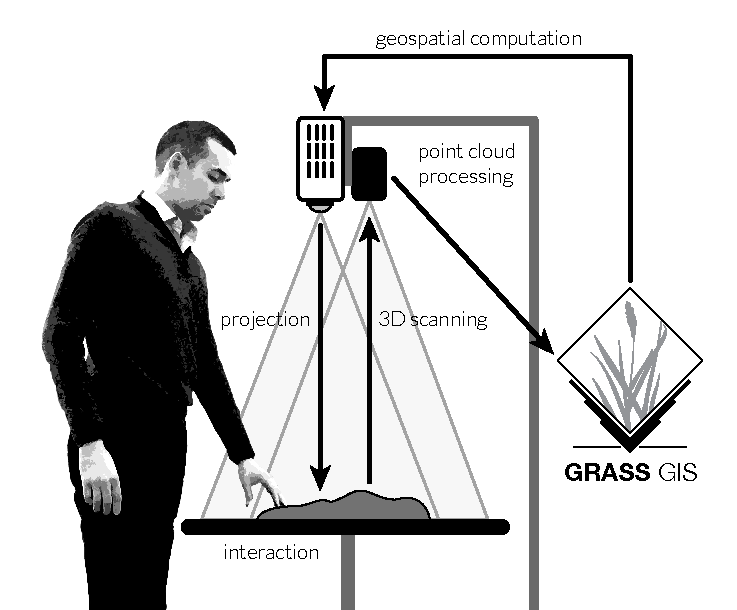
\includegraphics{images/system_schema_2.pdf}}
\caption{Caption.}
\label{fig:system_schema}
\end{figure}

% Modes of interaction
\paragraph{Modes of interaction}

% Fabrication and materiality

% Applications
\paragraph{Applications}

\subsection{Coupling experiment}

%Psychometric tests of spatial ability -- the application of spatial thinking -- for example study spatial visualization and mental rotation \citep{Uttal2013,Uttal2013a,Ormand2014}.
%We, however, do not just see space -- we also feel it; we use our bodies to feel size, shape, and volume. 
%Space need not be imagined to be transformed -- haptic feedback about space informs subconscious pragmatic representations that rapidly generate action \citep{Jeannerod1997}. Spatial thinking can be embodied.


\subsection{Analytics experiment}

\subsection{Case studies}

%Coffee \& Viz
Coffee \& Viz.
Scientific gaming: Structured problem solving with rules, challenging objectives, and scoring

\section{Results}

\section{Discussion}

\section{Future work}

% Cognitive science

% Real-time robotic fabrication

\section{Conclusion}

% Vision





%\section{...}
%% label
%\label{sec:examples}
%
%% Head 2
%\subsection{Head 2}
%
%% Head 3
%\subsubsection{Head 3}
%
%% Head 4
%\paragraph{Head 4}
%
%% quote
%\begin{quote}
%``\ldots".
%\end{quote}
%
%% itemize
%\begin{itemize}
%\item \ldots .
%\item \ldots .
%\item \ldots .
%\end{itemize}
%
%% footnote
%\ldots \footnote{...} 
%
%% enumerate
%\begin{enumerate}
%\item \ldots .
%\item \ldots . 
%\item \ldots .
%      \begin{enumerate}
%      \item \ldots .
%      \item \ldots .
%      \end{enumerate}
%\end{enumerate}
%
%% Enunciations
%\begin{definition}[...]...
%\end{definition}
%
%Table~\ref{tab:one}. 
%% Table
%\begin{table}%
%\tbl{...\label{tab:one}}{%
%\begin{tabular}{|l|l|}
%\hline
%...   & ...\\\hline
%...    & ...\\\hline
%\end{tabular}}
%\end{table}%

% Appendix
\appendix
\section*{APPENDIX}
\setcounter{section}{1}
In this appendix \ldots
\appendixhead{HARMON}

% Acknowledgments
\begin{acks}
\ldots
\end{acks}

% Bibliography
\bibliographystyle{ACM-Reference-Format-Journals}
\bibliography{tangible_topography.bib}

% History dates
%\received{}{}{}

% Electronic Appendix
\elecappendix

\medskip

\section{...}

\ldots

\end{document}



